\documentclass[qo.tex]{subfiles}

\begin{document}
\part{Quantum Theory In Condensed Matter}
\chapter{Bose-Einstein Statistics}
\section{Statistical Ensembles}
In statistical mechanics, one frequently formally considers $N$ copies of the system under consideration. 
Such an assembly is a \emph{statistical ensemble.}
\begin{itemize}
    \item In the \emph{microcanonical ensemble}, each copy has the same total poarticle number $N$ and total energy $U$.
    \item In the \emph{canonical ensemble}, each copy has the same total particle number $N$, however the total energy may fluctuate. 
        The system is considered to be in equilibrium with an external heat bath (maintaining a constant temperature $T$.
    \item In the \emph{grand canonical ensemble}, the total particle number and the total energy may fluctuate. 
        The system is considered to be in equilibrium with an external heat bath, and a particle bath (maintaining a constant chemical potential $\mu$).
\end{itemize}
We are generally interested in macroscopic systems of an effectively infinite number of particles, and may take the \emph{thermodynamic limit} $V\to\infty$ in which the particle density $n=N/V$ is held constant. 
The thermodynamic predictions of the three ensembles are then identical, and it is usually more convenient to use the grand canonical ensemble. 
If the $N$-body quantum states of $N$ quantum particles have energy $E_n^{(N)}$ for $n=1,2,\dots$, then in the grand canonical ensemble, each state occurs with probability
\begin{align}
    P_n^{(N)} &= \frac{1}{Z}\exp\left(-\frac{1}{k_BT}\left[E_n^{(N)}-\mu N\right]\right),
    \text{ where } Z = \sum_{N,k} \exp\left(-\frac{1}{k_BT}\left[E_n^{(N)}-\mu N\right]\right)
\end{align}
is the \emph{grand partition function.}

\section{Particle with Periodic Boundary Conditions}
Consider a point particle of mass $m$ moving within a volume $V=L_xL_yL_z$, where $L_i$ are lengths in the $i=x,y,z$ directions. 
The Hamiltonian 
\begin{equation}
    \hat{H} = \frac{1}{2m}\left(\hat{p}_x^2+\hat{p}_y^2+\hat{p}_z^2\right),
\end{equation}
and the eigenstates of the momentum operator $\hat{p}=(\hat{p}_x,\hat{p}_y,\hat{p}_z)$ are also eigenstates of $\hat{H}$ (subject to periodic boundary conditions).
In the \emph{position representation}, they take the form of plane waves:
\begin{align}
    \psi_k(\vr) = \frac{1}{\sqrt{V}}e^{i\unl{k}\cdot\vr}, \text{ where } \unl{k} = \left(\frac{2\pi n_x}{L_x},\frac{2\pi n_y}{L_y},\frac{2\pi n_z}{L_z}\right).
\end{align}
The differences in $k$ between neighbouring eigenstates are $2\pi/L_i$, in the $i=x,y,z$ directions.
The $k$-space density of the available states is therefore
\begin{align}
    \rho(\unl{k}) = \frac{L_xL_yL_z}{(2\pi)^3} = \frac{V}{(2\pi)^3}.
\end{align}

\section{Spherical Shells in k}
We divide up $k$-space into thin concentric shells. 
A shell of radius $k_S$ and thickness $\delta k_S$ has volume $4\pi k_S^2\delta k_S$, and therefore contains $M_S$ states, where
\begin{align}
    M_S &= 4\pi k_S^2\delta k_S\rho(\unl{k}) = 4\pi k_S^2\delta k_S \frac{V}{(2\pi)^3}.
\end{align}
Each such quantum state has energy $\e_S=\hbar^2k_S^2/2m$, from which we can determine an energy increment $\delta\e_S=(\hbar^2/m)k_S\delta k_S$.
Hence, the number of available states between energies $\e_S$ and $\e_S+\delta\e_S$ is
\begin{align}
    M_S = Vg(\e_S)\delta\e_S, \text{ where } g(\e) = \frac{m^{3/2}}{\sqrt{2}\pi^2\hbar^3}\e^{1/2}
\end{align}
is the (energy) density of states per unit volume. 
\emph{All states on a given shell have the same energy.}

\section{Thermal Equilibrium and the Bose-Einstein Distribution}
Consider an \emph{ideal Bose gas}, i.e. a system of many identical, non-interacting bosons, e.g. in a box subject to periodic boundary conditions. 
In \emph{thermal equilibrium}, the particles are distributed so that the occupation numbers $N_S$ in each shell of energy $\e_S$ maximise the total entropy. 
This yields the \emph{Bose-Einstein distribution:}
\begin{align}
    f_{BE}(\e) = \frac{1}{e^{(\e-\mu)/k_BT}-1}.
\end{align}

\section{Particle Density in the Thermodynamic Limit}
Using the Bose-Einstein distribution in Eq (1.7), the total number of particles in a volume $V$ (subject to periodic boundary conditions) is
\begin{align}
    N &= \sum_{\unl{k}}\frac{1}{e^{(\e_{\unl{k}}-\mu)/k_BT}-1}.
\end{align}
Taking the thermodynamic limit $V\to\infty$, the possible $\unl{k}$ values tend to a continuum, and we replace the sum $\sum_{\unl{k}}$ with an integral $\int\rho(\unl{k})\,dk_x\,dk_y\,dk_z \equiv \int\rho(\unl{k})\,d^3k = [V/(2\pi)^3]\int\,d^3k$.
Hence
\begin{align}
    N &= \frac{V}{(2\pi)^3}\int \frac{d^3k}{e^{(\e_{\unl{k}}-\mu)/k_BT}-1} \implies n \equiv \frac{N}{V} = \frac{1}{(2\pi)^3}\int \frac{d^3k}{e^{(\e_{\unl{k}}-\mu)k_BT}-1}.
\end{align}
Recalling $V/(2\pi)^3\,d^3k = [V/(2\pi)^3]4\pi k^2\,dk = Vg(\e)\,d\e$, then in terms of the density of states per unit volume, $g(\e)$,
\begin{align}
    n = \int \frac{g(\e)\,d\e}{e^{(\e_{\unl{k}}-\mu)/k_BT}-1}.
\end{align}

\chapter{Bose-Einstein Condensation}
\section{Particle Density in Terms of the Fugacity}
Using the fugacity $z\equiv e^{\mu/k_BT}$ and $x\equiv \e/k_BT$, we can rewrite the particle density $n$ as
\begin{align}
    n &= \frac{(mk_BT)^{3/2}}{\sqrt{2}\pi^2\hbar^3}\ofnt \frac{ze^{-x}}{1-ze^{-x}}x^{1/2}\,dx.
\end{align}
Taylor expanding $(1-ze^{-x})^{-1}$ around $ze^{-x}=0$, we deduce the identity
\begin{align}
    ze^{-x}(1-ze^{-x})^{-1} &= ze^{-x}\left(1+ze^{-x}+z^2e^{-2x} + \dots\right) = \sum_{j=1}^\infty z^je^{-jx}.
\end{align}
As $x>0$, this expansion is convergent for $z<1$, and we can evaluate the integral over $x$ using:
\begin{align}
    \ofnt e^{-jx}x^{1/2}\,dx &= \frac{1}{j^{3/2}}\underbrace{\ofnt e^{-y}y^{1/2}\,dy}_{\equiv \Gamma(3/2)} = \frac{1}{j^{3/2}}\frac{\sqrt{\pi}}{2}.
\end{align}
This implies 
\begin{align}
    n &= \left(\frac{mk_BT}{2\pi\hbar^2}\right)^{3/2}g_{3/2}(z), \text{ where } g_{3/2}(z) = \sum_{j=1}^\infty \frac{z^j}{j^{3/2}}.
\end{align}
We therefore need to know something of the properties of $g_{3/2}(z)$ to evaluate the particle density $n$.

\section{Properties of g}
The series defining $g_{3/2}(z)$ converges when $|z|<1$, and diverges when $|z|>1$.
At $z=1$, it is just convergent:
\begin{align}
    g_{3/2}(1) &= \zeta(3/2) = 2.612, \text{ where } \zeta(s) \equiv \sum_{j=1}^\infty \frac{1}{j^s}
\end{align}
is the Riemann zeta function.
The derivative of $g_{3/2}(z)$, however, is infinite at $z=1$, since
\begin{align}
    \frac{d}{dz}g_{3/2}(z)\bigg|_{z=1} &= \frac{1}{z}\sum_{j=1}^\infty \frac{z^j}{j^{1/2}}\bigg|_{z=1} = \sum_{j=1}^\infty \frac{1}{j_{1/2}}
\end{align}
diverges.
With these limiting values, we can make a sketch of $g_{3/2}(z)$ for $0\leq z\leq1$:
\begin{figure}[H]
    \centering
    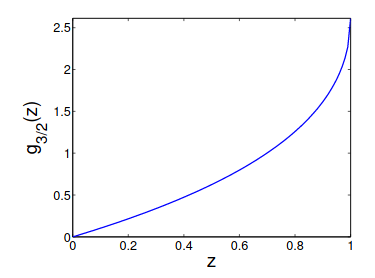
\includegraphics[scale=0.7]{g32.png}
\end{figure}

\section{Critical Temperature}
We can invert Eq (2.4) to get 
\begin{align}
    g_{3/2}(z) &= \left(\frac{2\pi\hbar^2}{mk_BT}\right)^{3/2}n.
\end{align}
If we are in a regime of high $T$ or low $n$, it follows that $g_{3/2}(z)$ must take a small value.
From the plot of $g_{3/2}(z)$ above, we see that this implies small $z$, which from the definition of $g_{3/2}(z)$ means we can approximate $g_{3/2}(z)\approx z$. 
Hence, recalling $z=e^{\mu/k_BT}$,
\begin{align}
    \mu &\approx -\frac32 k_BT\ln\left(\frac{mk_BT}{2\pi\hbar^2n^{2/3}}\right),
\end{align}
i.e., the chemical potential is negative. \\
As $n$ is fixed, it follows from Eq (2.4) that as $T$ is lowered (but assumed $T>0$), $z$ must increase, with maximum finite value of $z=1$, i.e. $\mu=0$.
It straightforwardly follows that this occurs at a \emph{critical temperature} (recalling $g_{3/2}(1)=2.612$) of 
\begin{align}
    T_C &= \frac{2\pi\hbar^2}{k_Bm}\left(\frac{n}{2.612}\right)^{2/3}.
\end{align}

\section{Macroscopic Occupation of the Ground State}
Recall that the Bose-Einstein distribution from Eq (1.7) predicts the occupation of $\e=\e_{\unl{k}=0}=0$ state to be 
\begin{align}
    N_0 &= \frac{1}{e^{-\mu/k_BT}-1}.
\end{align}
Hence, $\mu=0\implies N_0\to\infty$ (Bose-Einstein condensation).
Recalling that we are in the thermodynamic limit ($N,V\to\infty$), what this actually means is that $n_0=N_0/V$ is some finite fraction of $n$.
Rewriting Eq (2.10) for large $N_0$, we obtain 
\begin{align}
    \mu &= -k_BT\ln\left(1+\frac{1}{N_0}\right) \approx -\frac{k_BT}{N_0}.
\end{align}
Hence, as $N_0\to\infty$, $\mu\to0$.
Therefore, below $T_C$, the chemical potential $\mu$ is effectively 0.

\section{Below the Critical Temperature}
Below $T_C$, we must take $\vk=0$ point into account separately, and so we set $\mu=0$ and modify Eq (1.8) to
\begin{align}
    N &= N_0 + \sum_{\vk\neq0}^\infty \frac{1}{e^{\e_{\vk}/k_BT}-1}.
\end{align}
Again, replacing the sum by an integral (excluding $\vk=0$), the particle density is given by 
\begin{align}
    n = n_0 + \frac{(mk_BT)^{3/2}}{\sqrt{2}\pi^2\hbar^3}\ofnt \frac{e^{-x}}{1-e^{-x}}x^{1/2}\,dx.
\end{align}
The integral is identical to that evaluated in Sec (2.1), and so for $T<T_C$, 
\begin{align}
    n &= n_0 + 2.612\left(\frac{mk_BT}{2\pi\hbar^2}\right)^{3/2}.
\end{align}
One speaks of a \emph{condensate density} $n_0$, and a \emph{normal density} $n_n$.
Using the definition of $T_C$ in Eq (2.9), the \emph{condensate fraction} can be compactly written as
\begin{align}
    \frac{n_0}{n} &= 1-\left(\frac{T}{T_C}\right)^{3/2}.
\end{align}
Hence, at $T=0$, all particles are in the ground state, but the proportion decreases to zero as $T\to T_C$ from below, and is zero above $T_C$.

\section{Discontinuity in Heat Capacity Implies Phase Transition}
The heat capacity can be obtained by differentiating the internal energy per particle $u$ while keeping the density $n$ constant:
\begin{align}
    C_V &= \frac{\p u}{\p T}.
\end{align}
The total internal energy $U$ can be determined by multiplying the density of states $g(\e)$ by the volume $V$ and the Bose-Einstein distribution $f_{BE}(\e)$, and then integrating the resulting total energy distribution, multiplied over $\e$, over all values of $\e$:
\begin{align}
    U &= V\ofnt \frac{\e g(\e)\,d\e}{e^{(\e-\mu)/k_BT}-1} = \frac{V(k_BT)^{5/2}m^{3/2}}{\sqrt{2}\pi^2\hbar^3}\ofnt \frac{ze^{-x}}{1-ze^{-x}}x^{3/2}\,dx.
\end{align}
To calculate the average energy per particle, 
\begin{align}
    u &= \frac{U}{N} \equiv \frac{U/V}{N/V},
\end{align}
we use the expression for $n$ in Eq (2.4) to determine (by similar methods as in Sec 2.1), for $T>T_C$,
\begin{align}
    \frac{U}{V} &= \frac{(k_BT)^{5/2}m^{3/2}}{\sqrt{2}\pi^2\hbar^3}\underbrace{\sum_{j=1}^\infty\frac{z^j}{j^{5/2}}}_{\equiv g_{5/2}(z)}\underbrace{\ofnt e^{-y}y^{3/2}\,dy}_{\equiv \Gamma(5/2)},\\
    u &= k_BT\frac{\Gamma(5/2)g_{5/2}(z)}{\Gamma(3/2)g_{3/2}(z)} = \frac{3k_BT}{2}\frac{g_{5/2}(z)}{g_{3/2}(z)},
\end{align}
where we have used the identity $\Gamma(t)=(t-1)\Gamma(t-1)$.
Note that $g_{5/2}(z)$ and $g_{3/2}(z) \to z$ as $z\to0$, and so $\mu\approx \frac32 k_BT$ when $T\gg T_C$, i.e. the classical result. \\
For $T<T_C$, we use $n$ as given by Eq (2.9), and determine
\begin{align}
    u &= \frac{3k_B}{2}\frac{T^{5/2}}{T^{3/2}_C}\frac{g_{5/2}(1)}{g_{3/2}(1)},
\end{align}
where $g_{5/2}(1)=\zeta(5/2)=1.342$.\\
For $T\gg T_C$, we obtain the classical result
\begin{align}
    C_V &= \frac{\p u}{\p T} \approx \frac32 k_B;
\end{align}
while for $T<T_C$,
\begin{align}
    C_V &+ \frac{15}{4}\frac{g_{5/2}(1)}{g_{3/2}(1)}\left(\frac{T}{T_C}\right)^{3/2}k_B.
\end{align}
When plotted as a function of $T$, the curves for $T<T_C$ and $T>T_C$ meet at a cusp (discontinuity in slope).
This implies that the free energy is not analytic at $T_C$, and so BEC is a true thermodynamic \emph{phase transition.}

\emph{doodle plot from visualiser}






\end{document}













